\documentclass{jsarticle}
\usepackage{url}
\usepackage{graphicx}

\title{経済物理学レポート}
\author{奥戸 嵩登 \thanks{国立総合研究大学院大学 複合科学研究科 情報学専攻}}

\begin{document}
	\maketitle
	\section{はじめに}
	本レポートでは,2020年1月3日時点の時価総額トップ10の暗号資産銘柄について2019年1月1日から2019年12月31日までの価格変動データを用いて,相関関係分析を行う.相関がある場合それぞれの銘柄の価格変動は相互依存関係があり,相関がない場合は独立した価格変動を行っていることがわかる.価格変動の独立性は分散投資を行う際の指標として有効である.	
	
	\section{暗号資産について}
	
	\subsection{概要}
	暗号資産とは,法定通貨や法定通貨建ての資産ではないインターネット上でやりとりできる財産的価値である\cite{cryptoassets}.
	暗号資産は2008年にサトシナカモトと称する人物が論文をネット上に公開し,その論文をもとに複数の開発者が暗号資産を開発したことから始まっている.2019年5月31日に仮想通貨から暗号資産への名称変更の法案が可決された.
	暗号資産はビットコインとアルトコインの2つに大別される.ビットコインは初めて財産的価値を持った電子通貨である.アルトコインはビットコインの基盤技術を参考にして開発されたコインのことを指す\cite{alto}.暗号資産の種類は2019 年10月30日時点で2,351種類存在する.暗号資産は販売所または取引所を介して入手することができる.それぞれの違いは仮想通貨を売買する相手が異なることである.販売所は販売会社が相手であるのに対し,取引所は個人を相手にする.
	\subsection{ICO}
	ICOとはInitial Coin Offeringの略称であり,新規仮想通貨公開という意味である.企業や団体などが資金を調達する目的で独自のコインを発行する.そのため企業や団体への期待や価格上昇への期待から,ICOで発行されたコインは購入される.新規公開株式IPOと似ているが,大きな違いとしては出資者に与えられる権利の有無である.株式を保有した場合,株主優待の享受や株主総会への出席といった権利が出資者へ与えられる一方,コインの場合,これらの権利が一切ない\cite{ico}.
	
	\subsection{暗号資産の値動き}
	暗号資産の価格形成は株価や為替などと基本は同じであり,需要と供給によって決定される.また,ニュースが価格へ影響を及ぼすことに関しても同様である.暗号資産にはストップ高・ストップ安のような値幅制限が設けられていない場合が多いため,急激な価格変動が起こりやすいという特徴がある.
	
	\section{分析}
	本章では,ネット上で公開されている暗号通貨の価格データを用いて,それぞれの銘柄がどのような相関関係を持っているかを分析する.分析手法に関して,経済物理学第7回講義資料の為替市場に適用している手法を用いる.はじめに相互相関行列のヒートマップ示す.次に相関係数を距離の公理を満たすように変数変換を行い,デンドログラムにより可視化する.デンドログラムにおいて,どのようなクラスタが形成されるかについても分析を行う.分析には\url{https://github.com/takato86/cryptocurrency_analysis}にあるコードを用いた.
	\subsection{データセット}
	暗号通貨市場の分析を提供しているWebサイトCoinGeckoから2020年1月3日時点の時価総額トップ10の暗号資産の2019月1日1日から2019年12月31日時点までの日毎の値動きをデータを取得した.2020年1月3日時点の時価総額トップ10の暗号資産は下記の通りである.
	
	\begin{enumerate}
		\item Bitcoin/BTC
		\item Ethereum/ETH
		\item XRP/XRP
		\item Tether/USDT
		\item Bitcoin Cash/BCH
		\item Litecoin/LTC
		\item EOS/EOS
		\item Binance Coin/BNB
		\item Bitcoin SV/BSV
		\item Cardano/ADA
	\end{enumerate}

	以上の2020年1月3日時点の時価総額トップ10名柄について,分析を行う.
	
	\subsection{結果}
	2019年1月1日から2019年12月31日までの暗号資産のトップ10銘柄それぞれの価格データを用い,時系列の価格変動を可視化し,相関行列をヒートマップで表す.変数変換後,デンドログラムを形成されたクラスタと共に示す.
	はじめに,時系列の価格の変動を図\ref{fig:price_series}に示す.暗号資産の価格差が大きいため,標準化をして可視化した.0~1の範囲になるようにMinMaxScalerを用い,標準化を行った.
	
	\begin{figure}
		\begin{center}
		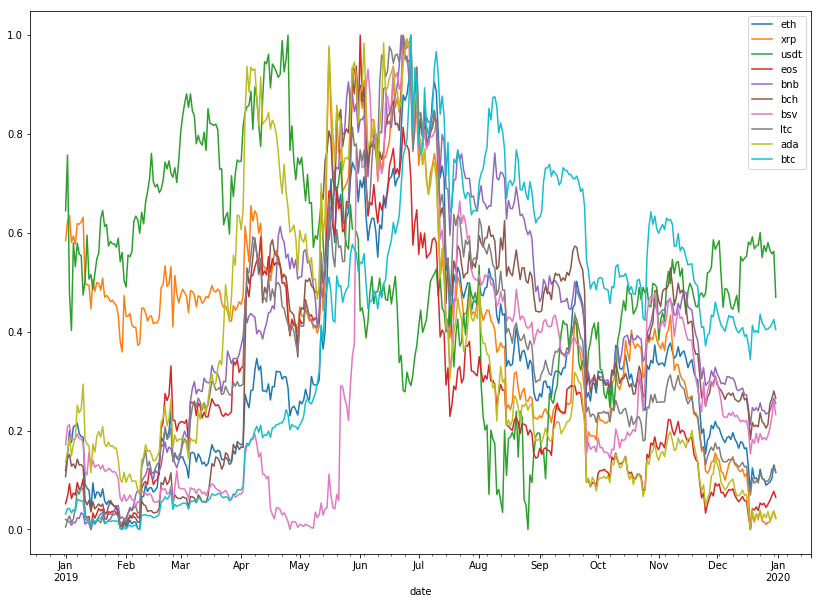
\includegraphics[bb=0.000000 0.000000 821.187048 604.137609, width=0.8\linewidth]{img/price_series.png}
		\caption{暗号資産の価格変動}
		\label{fig:price_series}
		\end{center}
	\end{figure}
	
	図\ref{fig:price_series}より,Tether/usdtの値動きが他の暗号資産と明らかに異なることがわかる.
	次に,銘柄ごとに1日の価格の増減データ系列を作成し,相関行列を算出する.相関行列のヒートマップを図\ref{fig:corr_matrix}に示す.
	
	\begin{figure}
		\begin{center}
		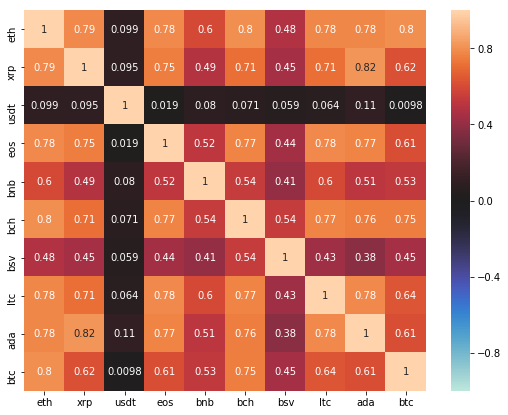
\includegraphics[bb=0.000000 0.000000 508.115737 415.094549, width=0.7\linewidth]{img/correlation_matrix.png}
		\caption{暗号資産間の変動の相関行列のヒートマップ}
		\label{fig:corr_matrix}
		\end{center}
	\end{figure}
	
	図\ref{fig:corr_matrix}より,Tether/usdtは他のどの暗号資産とも相関は見られなかった.Ethereum/ethはTether/usdtとBitcoin Cash/bch,Binance/bnbを除く他の7つの暗号資産とかなり強い正の相関があった.Bitcoin Cash/bchとはやや強い正の相関があるという結果であった .
	次に,クラスタリング の結果をデンドログラムで示す.相関係数は距離の公理を満たさないため下記の式で距離の公理を満たすように変数変換を行う.変数変換によって,正の相関が強いほど短い距離になる.
	$$
	d_{ij} = \sqrt{2(1-\rho_{ij})}
	$$
	$i, j$は暗号資産,$\rho_{ij}$は暗号通貨$i$と$j$の相関係数を示す.
	図\ref{fig:dendro}にデンドログラムを示す.
	
	\begin{figure}
		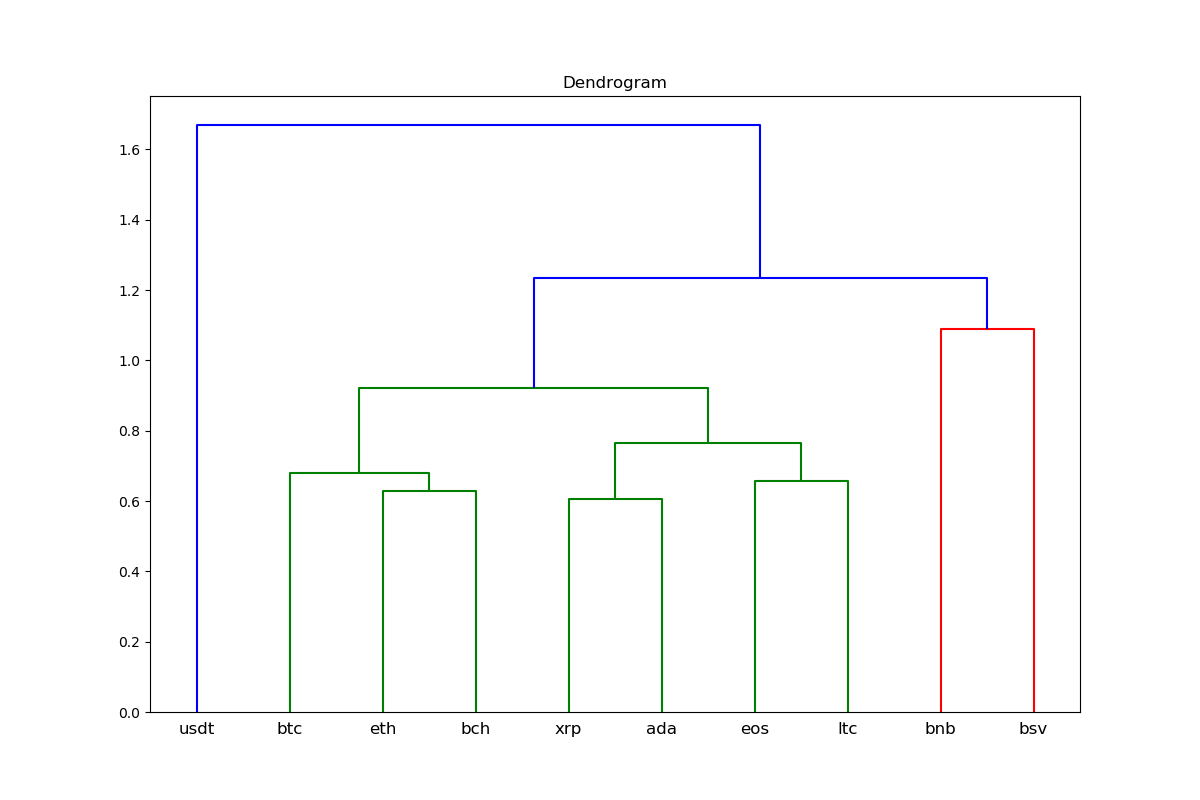
\includegraphics[bb=0.000000 0.000000 864.001728 576.001152, width=\linewidth]{img/2019-01-01_2019-12-31_dendrogram.png}
		\caption{デンドログラム}
		\label{fig:dendro}
	\end{figure}
	
	図\ref{fig:dendro}において,それぞれの色が銘柄が属するクラスタを表す.3つのクラスタが形成されていることがわかる.Tether/usdtのみのクラスタ,Binance Coin/bnbとBitcoin SV/bsvのクラスタ,それ以外の7銘柄のクラスタがそれぞれ形成された.
	\subsection{考察}
	図\ref{fig:dendro}において,単一でクラスタとなったTether/usdtにおいて考察をする.図\ref{fig:corr_matrix}より,Tether/usdtは他の暗号資産との無相関である暗号資産であった.Tether/usdtはペッグ通貨と呼ばれる他の通貨の価値と連動している暗号資産である\cite{tether}.1 usdtは1 USDで固定されており,米ドルと同価値に固定されているという特徴を持つコインである.他の暗号資産との相関が無かったことから,暗号資産は米ドルの価格変動との相関がないことがわかる.
	図\ref{fig:dendro}の最も大きいクラスタについて考察を行う.Bitcoin Cash/bch\cite{bch}とLitecoin/ltc\cite{ltc}はBitcoin/btcからハードフォークされた銘柄である.これら3名柄は最も大きいクラスタに属している.次に各銘柄がどの銘柄と強く相互依存しているかを明らかにするために,これらの暗号資産の大域最小木を図\ref{fig:mst} に示す.
	
	\begin{figure}
		\begin{center}
			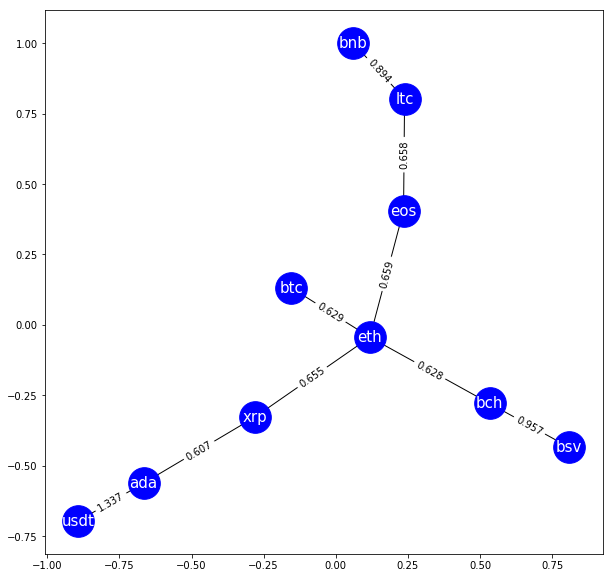
\includegraphics[bb=0.000000 0.000000 613.139660 578.131686, width=0.5\linewidth]{img/mst.png}
			\caption{全域最小木}
			\label{fig:mst}
		\end{center}
	\end{figure}
	
	
	図\ref{fig:mst}より,最大のクラスタに属する4つの銘柄はEthereum/ethの価格変動と強く相互依存している.10名柄のうち,暗号資産開発のためのプラットフォームを提供する企業から発行されている銘柄はEthereum/eth\cite{eth},XRP/xrp\cite{xrp},EOS/eos\cite{eos}であり,これらが強く結びついていることがわかる.
	次に,Binance Coin/bnbとBitcoin SV/bsvで構成されるクラスタについて考察する.図\ref{fig:corr_matrix}より,両者はEthereum/ethに対してTether/usdtを除くの他の銘柄に比べ正の相関が小さかった.Binance Coin/bnbとBitcoin SV/bsvの相互相関係数の大きさは0.41であり他の銘柄との相関係数と比べても平均的である.このことから,両者ともEthereum/ethとの相関が比較的小さかったため,同じクラスタになったと考えられる.Binance Coin/bnbは暗号資産の取引市場を運営するBinanceから発行されたコインであり,プラットフォームを運営するEthereum/ethとは異なる特徴を持つため,他の銘柄に比べて相関係数が低くなったと考えられる.Bitcoin SV/bsvはBitcoin Cash/bchからハードフォークされた銘柄である\cite{bsv}.したがって起源を辿るとBitcoin/btcに行き着く.しかしながら,Bitcoin/btcから直接ハードフォークされたBitcoin Cash/bchとLitecoin/ltcに比べて相関係数が低い結果であった.ハードフォークを繰り返すことで知名度が落ち,参加している投資家の質が上がっためと考えられる.
	
	\section{結論}
	本レポートでは,2019年1月1日から12月31日までの間で,2020年1月3日時点で時価総額トップ10の暗号資産銘柄の価格変動データを用いて,銘柄間の相関関係を分析した.分析結果より,ペッグ通貨であるTether/usdtとそれ以外の銘柄の価格変動は相互依存しないことが明らかになった.ペッグ通貨以外の銘柄では,Ethereum/ethの価格変動に強く依存するクラスタと比較的弱く依存するクラスタに分かれた.Ethereum/ethの価格変動に強く依存するクラスタには,プラットフォームを運営する企業が発行する銘柄が含まれていた.また,Bitcoinからハードフォークされた銘柄も同じクラスタに含まれていた.一方で,Bitcoin/btcを起源にもつBitcoin SV/bsvは異なるクラスタに属していた.Bitcoin/btcからハードフォークを重ねていくごとに知名度が落ち,参加する投資家の質が変化したことにより,価格変動の相互依存性を低下させたことが考えられる.今後の分析項目として,暗号資産の発行元が運営するサービスが価格変動の相互依存性に影響するかどうかや,ハードフォーク元とハードフォーク先の価格変動の相互相関関係を事例を増やして分析することが挙げられる.
	
	\begin{thebibliography}{5}
		\bibitem{cryptoassets} 暗号資産(仮想通貨)の利用者のみなさまへ,金融庁,\url{https://www.fsa.go.jp/policy/virtual_currency/index.html},2020/1/4参照.
		\bibitem{alto} アルトコイン,bitbank,\url{https://bitbank.cc/glossary/altcoin},2020/1/4参照.
		\bibitem{ico} ICOとは?初心者に解説する買い方とメリット・デメリット,コインチェック,\url{https://coincheck.com/ja/article/262},2020/1/4参照.
		\bibitem{coingecko} CoinGecko,CoinGecko,\url{https://www.coingecko.com/ja},2020/1/4参照.
		\bibitem{tether} 仮想通貨テザー(Tether/USDT)とは?米ドルと同じ価値を持つ仮想通貨を徹底解説,CoinOtaku,\url{https://coinotaku.com/posts/1585},2019年1/5参照.
		\bibitem{eth} Ethereum,Ethereum, \url{https://ethereum.org/ja/},2020年2月17日参照.
		\bibitem{ltc} ライトコイン,Wikipedia,\url{https://ja.wikipedia.org/wiki/ライトコイン},2020年2月17日参照.
		\bibitem{bch} ビットコインキャッシュ(BitcoinCash/BCH)とは?特徴やビットコインとの違いを徹底解説,Coincheck,\url{https://coincheck.com/ja/article/38},2020年2月17日参照.
		\bibitem{xrp} XRP,Ripple,\url{https://ripple.com/xrp/},2020年2月17日参照.
		\bibitem{eos} 仮想通貨EOS(イオス)の特徴、価格、取引所、将来性は?,Bitdays,\url{https://bitdays.jp/blockchain/cryptocurrency/eos/},2020年2月17日参照.
		\bibitem{bsv} ビットコインSV(BSV)とは?ビットコインABCとの違いや将来性は?,Coincheck,\url{https://coincheck.com/ja/article/266},2020年2月17日参照.
	\end{thebibliography}
\end{document}